\section{Optimization}
\subsection{Fibonacci - Cutoff}
  One possible optimization used in the BOTS benchmarks is implementing a cutoff option.
  This can be achieved by using if clause which is provided by the task directive as it is described in \cite{MKlemm.2018}.
  In case this clause evaluates to false no task will be spawned and the execution continues with the function call in a normal sequential way.
  The cutoff value is used to specify at which level the tasking spawning has to be stopped.
  A level parameter is added to the Fibonacci function and increased every recursive call.
  In case the level parameter is equal or greater than the cutoff value, the Fibonacci algorithm will be continued sequentially without spawning tasks. 
  Table \ref{tab:cutoff} shows the results without a cutoff and with a cutoff level equal to eight.
  The mean values of 100 runs are \(2057.34\) ms and \(394.87\) ms for OpenMP without and with a cutoff.
The average measurements for HPX are \(237491.49\) ms without and \(5267.67\) ms with cutoff.
It can be seen that the HPX implementation benefits more by the cutoff.
HPX speeds up by a ratio of approximately \(45\) and the OpenMP implementation speeds up only by \(5\).

\begin{table}
\centering
\caption{Execution times of the Fibonacci algorithm with cutoffs in milliseconds}
\begin{tabular}[h]{|l|c|c|}
\hline
 & With Cutoff & Without Cutoff \\\hline
OpenMP & \(2057.34\) ms & \(394.87\) ms \\\hline
HPX & \(237491.49\) ms & \(5267.67\) ms \\\hline
\end{tabular}
\label{tab:cutoff}
\end{table}

\subsection{OpenMP - untied / tied Tasks}
  Another optimization approach might be to see if there is a difference in using tied or untied tasks.
  Untied tasks improve the load balancing as each free thread can start executing a task which is ready to be executed.
  The disadvantage of untied tasks is that the data is not always available locally.
  This means in case a thread wants to execute a ready task which is not created by it, the data and context has to be transferred to new execution location.
  
\begin{figure}[h]
	\centering
	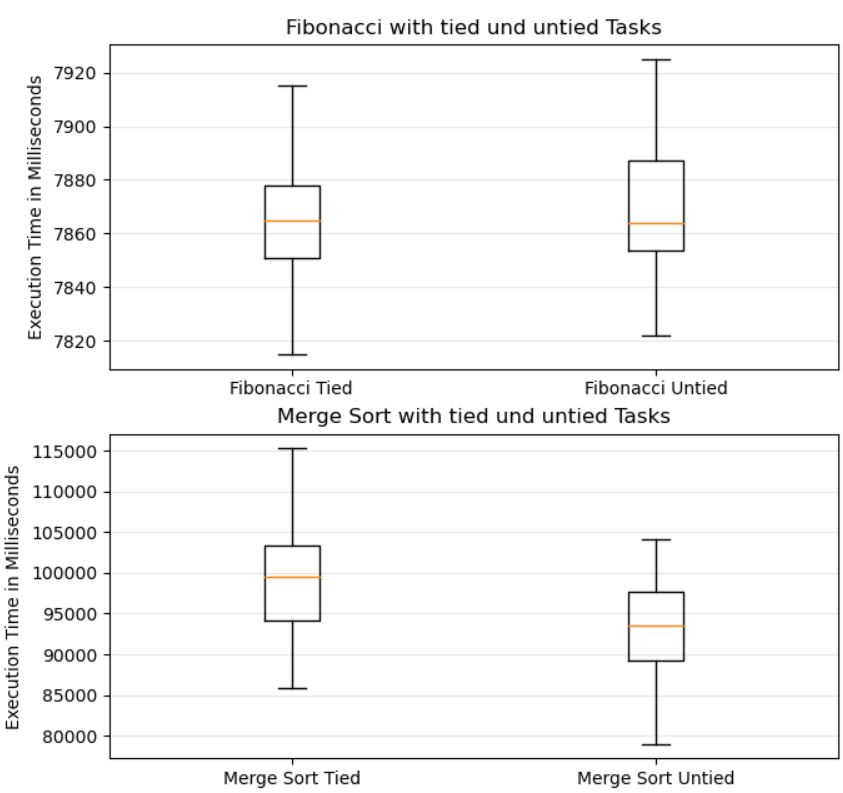
\includegraphics[width=0.45\textwidth]{figures/tied.JPG}
	\caption{Execution times of Fibonacci and Merge Sort with tied and untied Tasks in OpenMP}
	\label{fig:tied}
\end{figure}

  This experiment is run on environment 1 calculating again the Fibonacci number of 22.
  As figure \ref{fig:tied} shows there is no significant difference in execution time for both algorithms.
  Using tied or united tasks may only have minor impacts.
  As already mentioned this is due to the trade of of data locality and load balancing. 
  
\subsection{HPX - Fibonacci Dataflow}
HPX provides further LCOs than just futures.
Another object which might be useful is the \textit{dataflow} object.
It is an object which is used to define dependencies in functions easily.
Dataflows take a function and its parameters when initialized and call the function when all of its parameters are available. 
This might be the case for example if parameters are returned by futures.
However, it is also possible to concatenate dataflow objects to create a dependent hierarchy.~\cite{TheSTEARGroup.2020}

This experiment compares the HPX Fibonacci implementation using two futures with an implementation utilizing dataflows and another Fibonacci implementation using \texttt{when\_all}.
The last approach follows the same concept as the dataflow implementation, but works without this object type.
\texttt{when\_all} takes futures as parameters and starts executing when the values of all futures are available.
For this implementation the example code of HPX is taken as reference.~\cite{HPXGitHub.2020}
The idea is to utilize the dataflow principle to avoid blocked tasks and increase the scheduling overhead.

\begin{figure}[h]
	\centering
	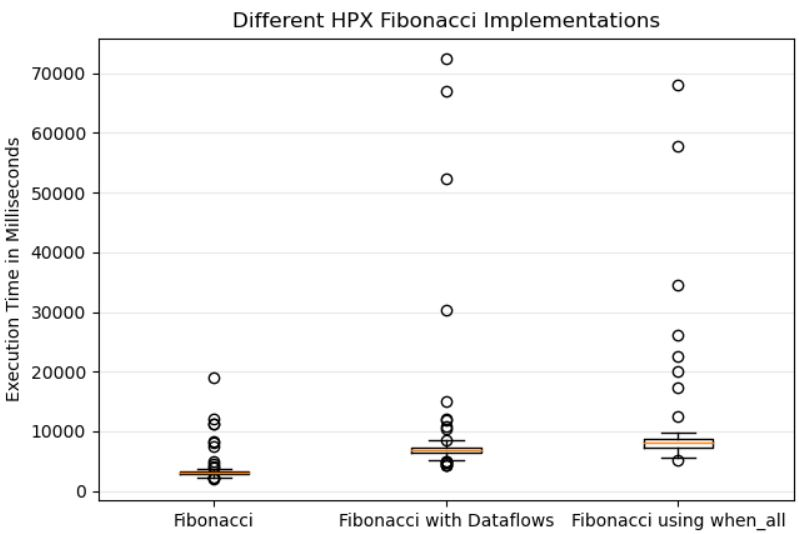
\includegraphics[width=0.45\textwidth]{figures/fibDataflow.JPG}
	\caption{Execution times of Fibonacci using HPX and different dataflow constructs}
	\label{fig:fib_dataflow}
\end{figure}

The average execution times of 100 runs on environment 3 for the 22\textsuperscript{nd} Fibonacci number's calculation are illustrated in figure \ref{fig:fib_dataflow}.
It can be seen that the normal Fibonacci implementation has the shortest execution times of these three.
This means that the dataflow principle cannot help avoiding scheduling overhead for HPX implementations.
Instead it produces additional overhead.


\subsection{HPX - Thread Scheduling Policies}
 The authors of \cite{hpxMP.2019} and \cite{TheSTEARGroup.2020} state different thread scheduling policies in HPX.
 However, not all of them are available at the HPX version used.
 Therefore only the policies used are explained.
 The experiment is run on environment 2.\\
 \textbf{local-priority} gives each operating system (OS) thread one queue they can pull their work from.
 Furthermore a high and low priority queue are created which is accessible by each OS thread.
 Work from these queues is only pulled in case the dedicated OS thread queue is empty.
 In doing so the high priority queue's work is taken first.
 Additionally, the local-priority policy is available in first-in-first-out (fifo) and last-in-first-out (lifo) version.\\
 \textbf{local} only maintains one queue per OS thread the work is put to and pulled from.\\
 \textbf{abp-priority} is similar to the local-priority policy.
 There are also a global high priority and low priority queue.
 However each OS threads owns a double ended lock free queue.
 Elements can be added and removed on both sides of this type of queue.
 Furthermore the abp-priority policy can also be used in fifo and lifo version.\\
 \textbf{static} has one queue per OS thread and tasks are distributed by round robin.
 In this policy no work stealing is available.\\
 \textbf{static-priority} is similar to local-priority as there are queues for each OS thread, high priority queues and low priority queues which can be accessed globally.
 In contrast to the local-priority policy the tasks are distributed by round robin and no work stealing is available.

\begin{figure}[h]
	\centering
	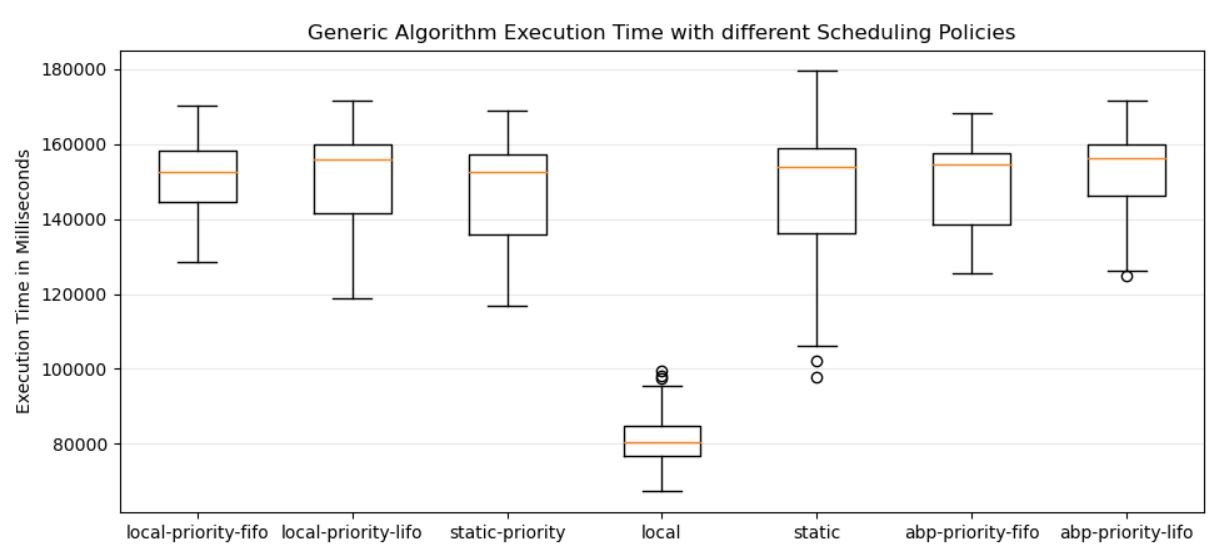
\includegraphics[width=0.45\textwidth]{figures/genSchedule.JPG}
	\caption{Execution times of the generic algorithm using different scheduling policies}
	\label{fig:gen_Schedule}
\end{figure}
\begin{figure}[h]
	\centering
	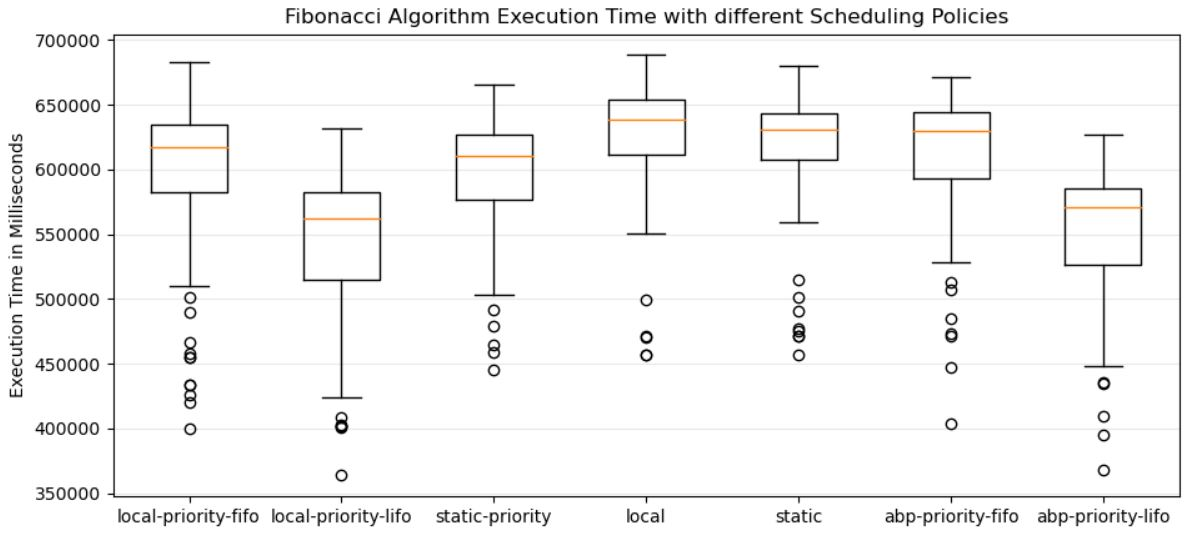
\includegraphics[width=0.45\textwidth]{figures/fibSchedule.JPG}
	\caption{Execution times of the Fibonacci algorithm using different scheduling policies}
	\label{fig:fib_Schedule}
\end{figure}
\begin{figure}[h]
	\centering
	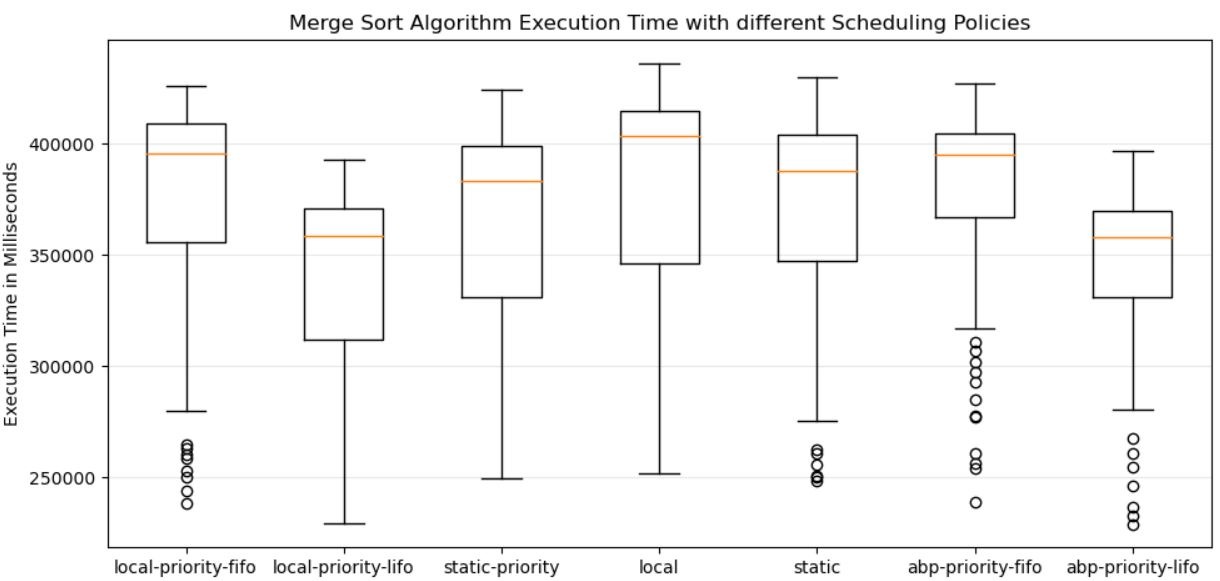
\includegraphics[width=0.45\textwidth]{figures/sortSchedule.JPG}
	\caption{Execution times of Merge Sort algorithm using different scheduling policies}
	\label{fig:sort_Schedule}
\end{figure}

The figures show the execution time of the three implemented algorithms with the previously explained thread scheduling policies.
The parameters are the same as stated in section \ref{sec:implem}.
Figure \ref{fig:gen_Schedule} is a boxplot diagram of the generic algorithm, figure \ref{fig:fib_Schedule} shows the execution times of the Fibonacci algorithm and figure \ref{fig:sort_Schedule} illustrates the execution times of merge sort.
It can be seen that the local policy accelerates the generic algorithm execution significantly compared to the other policies.
This may be because it produces little overhead as it does not have to maintain priority queues.
The significant difference to the static scheduling policy is that, when using the local policy, tasks are not distributed via round robin and task stealing is allowed.
These facts may lead to a better load balancing although the task size does not vary much.
The other two algorithms show no significant different in the policies.
However a trend can be seen as the mean values of the lifo policies show a shorter execution time in all cases.
This may be due to the fact that Fibonacci and merge sort create a task hierarchy in which the early created tasks are suspended till the end.

\subsection{Generic Algorithm - Number of Tasks}
For a better comparison of the three algorithms, various task sizes might be used.
The generic algorithm allows to adjust task sizes by parameters.
The second environment is taken for this test run in which tasks sizes ranging from 10 elements to 500 elements per task.
The total number of elements in the arrays \(1,048,576\) and the arrays are computed 50 times.
\begin{figure}[h]
	\centering
	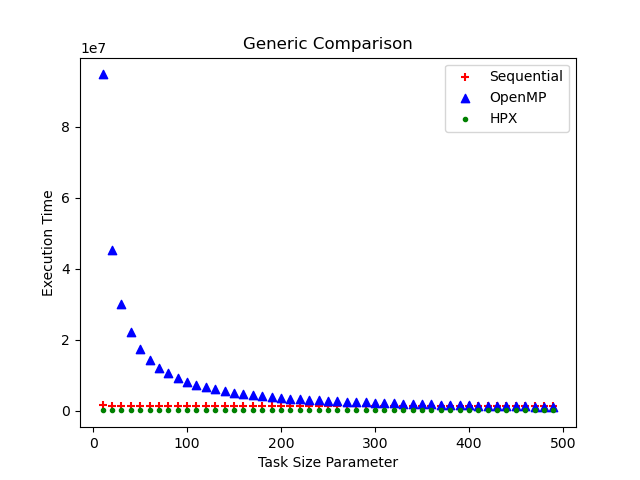
\includegraphics[width=0.45\textwidth]{figures/genericComp.png}
	\caption{Execution times of generic algorithm with various task sizes}
	\label{fig:genComp}
\end{figure}

\begin{figure}[h]
	\centering
	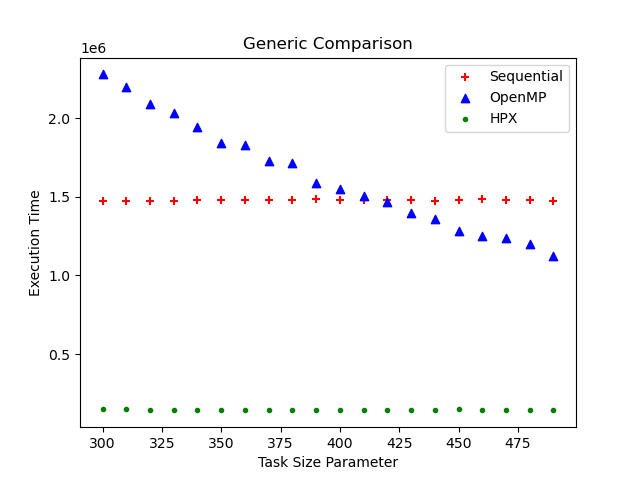
\includegraphics[width=0.45\textwidth]{figures/genericCompLast.png}
	\caption{Execution times of generic algorithm with biggest task sizes}
	\label{fig:genComp_Last}
\end{figure}

Figure \ref{fig:genComp} illustrates the execution time for all three elements.
The mean value of 50 measurements is taken.
It can be seen that the sequential and HPX implementation are quite constant.
In contrast, OpenMP takes more time when the task size is rather small and reaches the execution time of the sequential version at a task size of 410.
If the task size is bigger OpenMP takes less time compared to the sequential implementation.
However, it cannot reach the times of the HPX implementation.
Figure \ref{fig:genComp_Last} shows the same data however only the task sizes greater and equal to 300.
Especially, the trends of OpenMP and the sequential version can be seen in detail.
Important to mention is that changing the task size in the generic algorithm does not increase the overall workload.
This can be seen at the sequential implementation.
Changing the task size does only increase or decrease the tasks which are created.
In contrast to the Fibonacci algorithm and merge sort, the generic algorithm does not create hierarchical dependencies.
Task synchronization is done when all elements of an array are calculated.
HPX benefits from that structure as the lightweight threads used produce less overhead when forking and joining.
The scheduling overhead is smaller than the benefit from the parallel execution and therefore HPX becomes faster than the sequential implementation.
The joining and forking overhead can be seen in the execution times of OpenMP.
OpenMP does have operating system threads and therefore produces more overhead having bigger amounts of tasks.
However, reaching a certain task size OpenMP also takes less time than the sequential execution of the generic algorithm.


\subsection{Generic Algorithm - Task Sizes}
As the previous example of the generic algorithm does only increase the amount of tasks used and not the overall workload, another approach is also implemented.
In this experiment the generic algorithm is adjusted to produce a squared workload per array element.
The workload can be adjusted by a parameter and varies in this experiment.
In contrast to the experiments before, each task does only contain one element.
This setup does allow to have a constant number of tasks with an option to increase or decrease the task size and overall workload.
In each task the elements value is multiplied a defined amount of times.
The parameter for defining this size is squared, which means that if the parameter is equal to 3 the element is multiplied 9 times.
Each time the value is multiplied by the number of that multiply calculation.
In the example before the first value will be multiplied by 1 and multiplied by 9 in the last calculation.
The sinus function is then applied on the results and all of them are summed up and copied to the next array.
This experiment is also run on environment two having the same array size as the experiment before.
The number of calculations starts with 1x1 and increases by 2 in each dimension.
The biggest task size reached is 21x21.
For the HPX version the local thread scheduling policy is used.
\begin{figure}[h]
	\centering
	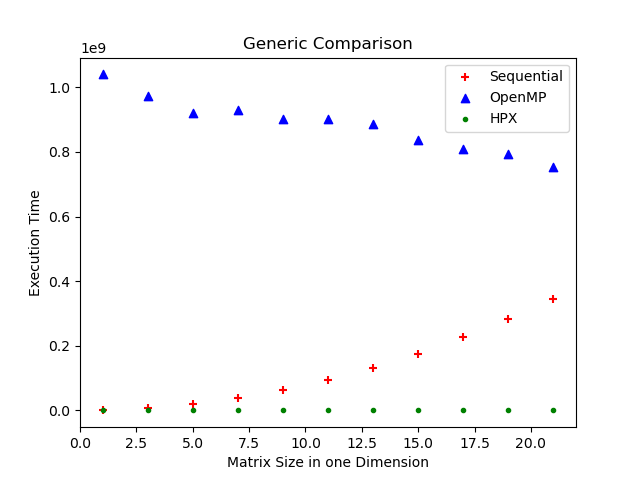
\includegraphics[width=0.45\textwidth]{figures/genericMatrix.png}
	\caption{Execution times of generic algorithm task matrices}
	\label{fig:genMatrix}
\end{figure}

Figure \ref{fig:genMatrix} shows the average execution time of 15 runs.
As already mentioned, the number of tasks are the same for all executions.
Increasing the matrix size increases the task size and overall workload as it can be seen by the sequential execution's curve.
The HPX execution time has a quite constant trend and OpenMP's curve decreases with an increasing task size, although the overall workload increases.


